% Options for packages loaded elsewhere
\PassOptionsToPackage{unicode}{hyperref}
\PassOptionsToPackage{hyphens}{url}
\PassOptionsToPackage{dvipsnames,svgnames,x11names}{xcolor}
%
\documentclass[
]{report}

\usepackage{amsmath,amssymb}
\usepackage{iftex}
\ifPDFTeX
  \usepackage[T1]{fontenc}
  \usepackage[utf8]{inputenc}
  \usepackage{textcomp} % provide euro and other symbols
\else % if luatex or xetex
  \usepackage{unicode-math}
  \defaultfontfeatures{Scale=MatchLowercase}
  \defaultfontfeatures[\rmfamily]{Ligatures=TeX,Scale=1}
\fi
\usepackage{lmodern}
\ifPDFTeX\else  
    % xetex/luatex font selection
\fi
% Use upquote if available, for straight quotes in verbatim environments
\IfFileExists{upquote.sty}{\usepackage{upquote}}{}
\IfFileExists{microtype.sty}{% use microtype if available
  \usepackage[]{microtype}
  \UseMicrotypeSet[protrusion]{basicmath} % disable protrusion for tt fonts
}{}
\makeatletter
\@ifundefined{KOMAClassName}{% if non-KOMA class
  \IfFileExists{parskip.sty}{%
    \usepackage{parskip}
  }{% else
    \setlength{\parindent}{0pt}
    \setlength{\parskip}{6pt plus 2pt minus 1pt}}
}{% if KOMA class
  \KOMAoptions{parskip=half}}
\makeatother
\usepackage{xcolor}
\setlength{\emergencystretch}{3em} % prevent overfull lines
\setcounter{secnumdepth}{-\maxdimen} % remove section numbering
% Make \paragraph and \subparagraph free-standing
\ifx\paragraph\undefined\else
  \let\oldparagraph\paragraph
  \renewcommand{\paragraph}[1]{\oldparagraph{#1}\mbox{}}
\fi
\ifx\subparagraph\undefined\else
  \let\oldsubparagraph\subparagraph
  \renewcommand{\subparagraph}[1]{\oldsubparagraph{#1}\mbox{}}
\fi


\providecommand{\tightlist}{%
  \setlength{\itemsep}{0pt}\setlength{\parskip}{0pt}}\usepackage{longtable,booktabs,array}
\usepackage{calc} % for calculating minipage widths
% Correct order of tables after \paragraph or \subparagraph
\usepackage{etoolbox}
\makeatletter
\patchcmd\longtable{\par}{\if@noskipsec\mbox{}\fi\par}{}{}
\makeatother
% Allow footnotes in longtable head/foot
\IfFileExists{footnotehyper.sty}{\usepackage{footnotehyper}}{\usepackage{footnote}}
\makesavenoteenv{longtable}
\usepackage{graphicx}
\makeatletter
\def\maxwidth{\ifdim\Gin@nat@width>\linewidth\linewidth\else\Gin@nat@width\fi}
\def\maxheight{\ifdim\Gin@nat@height>\textheight\textheight\else\Gin@nat@height\fi}
\makeatother
% Scale images if necessary, so that they will not overflow the page
% margins by default, and it is still possible to overwrite the defaults
% using explicit options in \includegraphics[width, height, ...]{}
\setkeys{Gin}{width=\maxwidth,height=\maxheight,keepaspectratio}
% Set default figure placement to htbp
\makeatletter
\def\fps@figure{htbp}
\makeatother

\makeatletter
\@ifpackageloaded{caption}{}{\usepackage{caption}}
\AtBeginDocument{%
\ifdefined\contentsname
  \renewcommand*\contentsname{Table of contents}
\else
  \newcommand\contentsname{Table of contents}
\fi
\ifdefined\listfigurename
  \renewcommand*\listfigurename{List of Figures}
\else
  \newcommand\listfigurename{List of Figures}
\fi
\ifdefined\listtablename
  \renewcommand*\listtablename{List of Tables}
\else
  \newcommand\listtablename{List of Tables}
\fi
\ifdefined\figurename
  \renewcommand*\figurename{Figure}
\else
  \newcommand\figurename{Figure}
\fi
\ifdefined\tablename
  \renewcommand*\tablename{Table}
\else
  \newcommand\tablename{Table}
\fi
}
\@ifpackageloaded{float}{}{\usepackage{float}}
\floatstyle{ruled}
\@ifundefined{c@chapter}{\newfloat{codelisting}{h}{lop}}{\newfloat{codelisting}{h}{lop}[chapter]}
\floatname{codelisting}{Listing}
\newcommand*\listoflistings{\listof{codelisting}{List of Listings}}
\makeatother
\makeatletter
\makeatother
\makeatletter
\@ifpackageloaded{caption}{}{\usepackage{caption}}
\@ifpackageloaded{subcaption}{}{\usepackage{subcaption}}
\makeatother
\ifLuaTeX
  \usepackage{selnolig}  % disable illegal ligatures
\fi
\usepackage{bookmark}

\IfFileExists{xurl.sty}{\usepackage{xurl}}{} % add URL line breaks if available
\urlstyle{same} % disable monospaced font for URLs
\hypersetup{
  pdftitle={🪖 The AI Battlefield},
  colorlinks=true,
  linkcolor={blue},
  filecolor={Maroon},
  citecolor={Blue},
  urlcolor={Blue},
  pdfcreator={LaTeX via pandoc}}

\title{🪖 The AI Battlefield}
\author{}
\date{2024-02-13}

\begin{document}
\maketitle

\chapter{The AI Battlefield Engineering - What You Need To
Know}\label{the-ai-battlefield-engineering---what-you-need-to-know}

This chapter is one person's opinionated overview of the ML/AI
Engineering reality, which may or may not be another person's reality.
The intention is to help you start asking the right questions and get
your ML Engineering needs met.

\section{Basics}\label{basics}

\subsection{What's important in the AI
race?}\label{whats-important-in-the-ai-race}

Training:

\begin{enumerate}
\def\labelenumi{\arabic{enumi}.}
\tightlist
\item
  How fast one can train a better model (first to market advantage)
\item
  How much \$\$ was spent (do we still have money left to pay salaries
  to talent after training?)
\end{enumerate}

Inference:

\begin{enumerate}
\def\labelenumi{\arabic{enumi}.}
\tightlist
\item
  Fast latency (users are used to msec response times and will leave if
  the response takes seconds)
\item
  Fast throughput (how many concurrent queries can be processed)
\item
  How much \$\$ is being spent per user (can we rent more GPUs to
  acquire more users and/or improve (1) and (2)?)
\end{enumerate}

\subsection{What are the needs of LLM
training?}\label{what-are-the-needs-of-llm-training}

\begin{enumerate}
\def\labelenumi{\arabic{enumi}.}
\tightlist
\item
  Fast compute massively dominated by matrix multiplications
\item
  Fast enough memory, IO, network and CPU to feed the compute
\end{enumerate}

Corollary: If when you buy or rent hardware you invest in the fastest
accelerators, but cheap out on any of the other components you wasted
\$\$ and you might not win the race as it'll take longer to train.

\subsection{What are the workhorses of
ML?}\label{what-are-the-workhorses-of-ml}

\begin{itemize}
\item
  An accelerator or a processing unit is what does most of the work.
\item
  Since ML does a lot of parallel processing
  (\href{https://en.wikipedia.org/wiki/Single_instruction,_multiple_data}{SIMD})
  GPUs were used at the beginning, but now you additionally have TPUs,
  IPUs, FPGAs, HPUs, QPUs, RDUs, etc. Recent CPUs are becoming used as
  accelerators as well, especially for inference.
\end{itemize}

\href{../compute/accelerator}{More details}.

\subsection{AI driving entities}\label{ai-driving-entities}

\begin{itemize}
\tightlist
\item
  AI companies - train models/build products around self-trained or
  trained-by-others' models, in-house research.
\item
  Academia - does massive research and write papers. Lots of new ideas
  are generated.
\item
  AI enthusiasts - lots of good will available, some pull
  resources/talents together to train open access models, with donated
  compute by HPCs and an occasional cloud, or a university cluster.
\item
  Entrepreneurs - lots of low hanging fruit to pick - creative reselling
  of services, making ML-driven apps, and using various ingenious
  combinations of available resources to create amazing outcomes.
\end{itemize}

\subsection{Information sharing}\label{information-sharing}

\begin{itemize}
\tightlist
\item
  It's very surprising that almost everybody involved in the domain of
  AI shares a lot of the discoveries with the community.
\item
  Surely, companies don't disclose all of their IP, but a lot of it does
  get shared in the form of knowledge or model weights
\item
  Companies that publish a lot of IP and models tend to attract higher
  quality talent.
\item
  Twitter seems to be the central platform where one must be to follow
  what's going on
\end{itemize}

\subsection{The AI bubble}\label{the-ai-bubble}

\begin{itemize}
\item
  The \href{https://en.wikipedia.org/wiki/Dot-com_bubble}{Dot-com
  bubble} occurred during 1995-2000. And a very similar situation is
  happening right now in the AI space.
\item
  There is a lot of money available to create new startups or boost the
  existing companies. It's relatively easy to raise millions of dollars.
\item
  As we are in the wild-wild-west stage of the AI industry it's very
  difficult to predict the future, and so pretty much anything goes as
  far as startup ideas go, as long as it sounds reasonable.
\item
  What distinguishes the AI bubble from the Dot-com bubble, is that one
  didn't actually need much money to operate a Dot-com company - most of
  the raised money went to marketing and some to staff, barely any to
  compute. AI companies need millions of dollars because training LLMs
  requires an insane amount of compute, and that compute is very
  expensive. e.g.~1x NVIDIA H100 costs \textasciitilde\$30k and a
  company may need 512 of those, which is \$15M (not counting the other
  hardware components and related costs)!
\end{itemize}

\section{ML Engineer's heaven and
hell}\label{ml-engineers-heaven-and-hell}

This is my personal LLM/VLM trainings-based heaven and hell. YMMV.

\subsection{ML Engineer's heaven}\label{ml-engineers-heaven}

\begin{enumerate}
\def\labelenumi{\arabic{enumi}.}
\item
  A well built HPC, or a full service cloud based cluster, where someone
  diligently and timely takes care of the hardware and the systems.

  I just need to bring my training software and do the training, which
  is already an insanely complicated job requiring special skills.
\item
  Lots of nodes available for exclusive unlimited use
\item
  Fast inter-node connectivity that doesn't bottleneck the accelerators
  and which isn't shared with other users
\item
  Huge local super-fast NVME based shared filesystem that can fit
  datasets and checkpoints
\item
  Barebones Linux w/ SLURM and minimal software to be able to launch
  training jobs
\item
  \texttt{sudo}er access to ease the work with a team of people
\end{enumerate}

\subsection{ML Engineer's hell}\label{ml-engineers-hell}

\begin{enumerate}
\def\labelenumi{\arabic{enumi}.}
\item
  A cloud or in-house cluster, where you have to do everything -
  sysadmining, replacing hardware, dealing with outages, etc. And to do
  the training on top of that.
\item
  A smallish slow shared filesystem (NFS?), with cloud to draw data from
  and checkpoint to
\item
  Slow inter-node leading to low accelerator utilization
\item
  Inter-node shared with other users which make the network erratic and
  unpredictable
\item
  Super-complicated cloud console with gazillion of screens and steps to
  set even simple things up
\item
  Not being able to swap out failing hardware fast
\item
  Needing to timeshare the nodes - with wait times between training jobs
\item
  Having other concurrent users who might use up the whole disk, leading
  to trainings crashing
\item
  Not being able to kill jobs others on the team started and went to
  sleep
\end{enumerate}

\section{Getting compute}\label{getting-compute}

There are 3 main choices to where one gets compute:

\begin{itemize}
\tightlist
\item
  Rent on the cloud
\item
  Get a timeshare on an HPC
\item
  Buy it
\end{itemize}

\subsection{Renting on the cloud}\label{renting-on-the-cloud}

This is currently the prevalent way of getting compute.

Pros:

\begin{itemize}
\tightlist
\item
  Easy to expand or contract the size of the cluster
\item
  Easy to upgrade from the old hardware generation to the new one in a
  few years
\item
  Cluster management could be easily outsourced
\end{itemize}

Cons:

\begin{itemize}
\tightlist
\item
  Expensive, unless you negotiate a long term (1-3 year) contract for
  hundreds of accelerators
\item
  You will be tempted to buy many tools and services that you may or may
  not need
\item
  You always get charged whether you use your cluster fully or not
\end{itemize}

\subsection{Using HPC}\label{using-hpc}

There aren't that many HPCs out there and so the amount of available
resources is limited.

Pros: - Managed for you - all you need is your software to do the
training and a bit of \href{../orchestration/slurm}{SLURM} know-how to
launch jobs - Often sponsored by the local government/university -
probably could get the job done for less \$\$ or even free (e.g.~we
trained \href{https://huggingface.co/bigscience/bloom}{BLOOM-176B} for
free on \href{http://www.idris.fr/eng/jean-zay/}{JeanZay HPC}!)

Cons: - needing to time share compute with other teams == short job
times with possible long wait times in between - could be difficult to
finish training quickly - The inter-node network is likely to be
unstable as it'll be used by other teams - Have to abide by the HPC's
rules (e.g.~no \texttt{sudo} access and various other rules to follow) -
In a way the HPC cluster will be what it'll be - you can't make the
network faster and often even getting some software installed can be
tricky.

\subsection{Buying hardware}\label{buying-hardware}

It's mainly universities that buy and build their own clusters, and some
big companies do that too.

Pros:

\begin{itemize}
\tightlist
\item
  If you can deploy the hardware 24/7 for more than a few years the
  total cost will be cheaper than renting
\item
  Easy to provide fast local storage - a good NVME raid would be much
  cheaper and faster than online storage
\end{itemize}

Cons:

\begin{itemize}
\tightlist
\item
  You're stuck with the outdated hardware just a few years after it was
  purchased - might be able to resell
\item
  Must buy more than needed - Hardware tends to break, especially when
  it's used 24/7, RMA could take weeks
\item
  Have to hire talent to manage the in-house solution
\item
  Have to figure out cooling, electric costs, insurance, etc.
\end{itemize}

\section{The needs of technology}\label{the-needs-of-technology}

\subsection{Can you feed the furnace fast
enough?}\label{can-you-feed-the-furnace-fast-enough}

Imagine a steam locomotive - the engine is great, but if the
\href{https://en.wikipedia.org/wiki/Fireman_(steam_engine)}{fireman}
isn't fast enough to shovel the coal in, the train won't move fast.

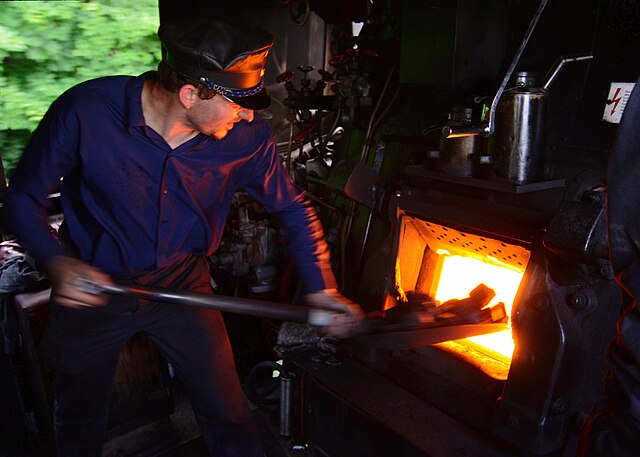
\includegraphics{images/640px-Baureihe52Heizer.jpg}

\href{https://commons.wikimedia.org/wiki/File:Baureihe52Heizer.jpg}{source}

This is the current state of ML hardware: The bottleneck is in moving
bits and not the compute.

\begin{itemize}
\tightlist
\item
  Accelerators get \textasciitilde2x faster every 2 years
  (\href{https://en.wikipedia.org/wiki/Moore\%27s_law}{Moore's law})
\item
  Network and memory are not! Already now both are compute bottlenecks
\item
  IO can be another bottleneck if your DataLoader has to pull data from
  the cloud
\item
  CPU is fine as long as it has enough cpu-cores for DataLoader workers,
  and main processes
\end{itemize}

Corollary: research the whole machine and not just its engine.

a crazy idea: the older GPUs might do fine if you can actually feed them
as fast as they can compute. And if you can get 3x of them at the same
cost as the next generation GPU you might finish training sooner and a
lower cost.

\subsection{TFLOPS}\label{tflops}

\begin{itemize}
\item
  Once you choose the architecture and the size of the model and how
  many tokens you want to train the model for you immediately know how
  much compute will be required to accomplish this goal. Specifically
  you can now calculate
  \href{../training/performance/README.md\#tflops-as-a-performance-metric}{how
  many floating point operations will be needed}.
\item
  All that is missing is comparing different compute providers to how
  many floating point operations their hardware can computes per secs
  (TFLOPS) and their cost per unit and now you can tell the total
  approximate cost of the training.
\end{itemize}

\begin{enumerate}
\def\labelenumi{\arabic{enumi}.}
\item
  Calculate the time needed to train given the TFLOPS of the considered
  solution:

  \texttt{total\_tflops\_required\ /\ tflops\_of\_this\_compute\_unit\ =\ time\_in\_seconds}

  Let's say it came to be 604800 secs or 7 days.
\item
  Look at the cost of using this compute solution for 7 days and now you
  know the total \$\$ to train this model.
\item
  Look at other proposals and calculate the same - chose the best
  option.
\end{enumerate}

\begin{itemize}
\tightlist
\item
  As mentioned earlier, time is of a huge importance, so you might still
  choose a more expensive solution if finishing the training sooner is
  important because you want to be first to market.
\end{itemize}

Unfortunately, this math is only partially correct because the
advertised peak TFLOPS are typically unachievable. The MFU section
delves into it.

\subsection{Model Flops Utilization
(MFU)}\label{model-flops-utilization-mfu}

As mentioned in the previous section, some (most?) vendors publish
unrealistic peak performance TFLOPS - they aren't possible to achieve.

Model Flops Utilization (MFU) is the metric that tells us how well the
accelerator is utilized. Here is how it is calculated:

\begin{enumerate}
\def\labelenumi{\arabic{enumi}.}
\tightlist
\item
  Measure the actual TFLOPS by calculating how many floating point
  operations a single training iteration takes and dividing that number
  by the number of seconds this iteration took.
\item
  Divide the actual TFLOPS by advertised TFLOPS to get the MFU
\end{enumerate}

Example: Let's say you're training in BFLOAT16 precision:

\begin{itemize}
\tightlist
\item
  If a single iteration requires 624 Tera floating point operations and
  it took 4 secs to run then we know that we get: \texttt{624/4=156}
  actual TFLOPS
\item
  now BF16@A100 is
  \href{https://www.nvidia.com/en-us/data-center/a100/}{advertised as
  312TFLOPS} so \texttt{156/312=0.5} gives us 50\% MFU.
\end{itemize}

Practically: - with NVIDIA GPUs if you're above 50\% MFU on a multi-node
setup with a large model you're already doing fantastic - recent
advancements in more efficient scalability solutions keep on increasing
MFU - slow networks and inefficient frameworks or untuned configuration
lower MFU

Therefore once you know the MFU you can now adjust the cost estimate
from the previous section. In the example there we said it'll take 7
days to train, but if MFU is 50\%, it means it'll take 14 days to train.

\subsection{Moving bits}\label{moving-bits}

Why can't the advertised TFLOPS achieved? It's because it takes time to
move data between accelerator memory and compute and additionally it
takes even more time to move data from disk and other gpus to the
accelerator's memory.

\begin{itemize}
\item
  There is not much can be done about the accelerator memory since its
  bandwidth is what it is - one can only write more efficient software
  to make data move faster to/from the accelerator - hint: fused and
  custom written kernels (like
  \href{https://pytorch.org/docs/stable/generated/torch.compile.html}{torch.compile}
  and \href{https://github.com/Dao-AILab/flash-attention}{flash
  attention})
\item
  If you only have a single GPU and the model fits its memory, you don't
  need to worry about the network - accelerator memory is the only
  bottleneck. But if you have \href{../training/model-parallelism}{to
  shard the model across multiple GPUs} network becomes the bottleneck.
\item
  Intra-node Network - is very fast, but difficult to take advantage of
  for large models -
  \href{../training/model-parallelism\#tensor-parallelism}{Tensor
  parallelism} and
  \href{../training/model-parallelism\#sequence-parallelism}{sequence
  parallelism} address part of this problem.
  (\href{../network/README.md\#intra-node-networking}{more}).
\item
  Inter-node Network - typically is too slow on most server setups -
  thus this is the key component to research! Efficient frameworks
  succeed to partially hide the comms overhead by overlapping compute
  and comms. But if comms take longer than compute, the comms are still
  the bottleneck. \hyperref[inter-node-network]{more}.
\item
  Storage IO is important primarily for feeding the DataLoader workers
  and saving the checkpoints. \hyperref[storage]{more}.

  \begin{enumerate}
  \def\labelenumi{\arabic{enumi}.}
  \tightlist
  \item
    Typically with enough DL workers the DataLoader adds very little
    overhead.
  \item
    While checkpoints are being saved the accelerators idle unless some
    async saving solution is used, so fast IO is crucial here
  \end{enumerate}
\end{itemize}

\section{Key hardware components}\label{key-hardware-components}

\subsection{Accelerators}\label{accelerators}

As of this writing here are the most common accelerators that can be
used for training, finetuning and inference ML models:

Widely available:

\begin{itemize}
\tightlist
\item
  NVIDIA A100 - huge availability across all clouds, but is already
  gradually being replaced by H100
\end{itemize}

Available, but locks you in:

\begin{itemize}
\tightlist
\item
  Google TPUs - fast! but the cost is a lock-in into a single vendor and
  cloud
\end{itemize}

Emerging to general availability:

\begin{itemize}
\item
  NVIDIA H100 - 2-3x faster than A100 (half precision), 6x faster for
  fp8
\item
  AMD MI250 \textasciitilde= A100 - very few clouds have them
\item
  AMD MI300 \textasciitilde= H100 - don't expect until 1.5-2 years from
  now to be GA
\item
  Intel Gaudi2 \textasciitilde= H100 - starting to slowly emerge on
  Intel's cloud
\item
  GraphCore IPU - very difficult to find, paperspace has them
\item
  Cerebras WaferScale Engine - available on Cerebras' cloud
\end{itemize}

\subsubsection{Accelerator
Interoperability}\label{accelerator-interoperability}

In general most (all?) accelerators are supported by major frameworks
like PyTorch or TensorFlow and the same code should run everywhere with
small modifications as long as it doesn't use any accelerator-specific
functionality.

For example, if your PyTorch application includes custom CUDA kernels
it'll only work on NVIDIA GPUs and may be on AMD MI-series.

\begin{itemize}
\item
  NVIDIA GPUs: all based on
  \href{https://developer.nvidia.com/cuda-toolkit}{CUDA}, which most
  training frameworks support. You can easily moved between different
  NVIDIA GPUs and most things would work the same.
\item
  AMD MI250/MI300: with PyTorch using
  \href{https://pytorch.org/blog/pytorch-for-amd-rocm-platform-now-available-as-python-package/}{ROCm}
  you can run most CUDA-based software as is. This is really the only
  inter-operable accelerator with the NVIDIA stack.
\item
  Gaudi2: if you use HF Transformers/Diffusers you can use
  \href{https://github.com/huggingface/optimum-habana}{optimum-habana}.
  If you use HF Trainer with NVIDIA GPUs it should be relatively easy to
  switch to train/infer on Gaudi2.
\item
  GraphCore IPU: can also be run via PyTorch via
  \href{https://github.com/graphcore/poptorch}{poptorch}
\item
  Cerebras: is also working on PyTorch support via
  \href{https://www.cerebras.net/blog/supporting-pytorch-on-the-cerebras-wafer-scale-engine/}{Cerebras
  Software Platform (CSoft) via XLA}.
\end{itemize}

Also in general most ML code could be compiled into cross-platform
formats like
\href{https://en.wikipedia.org/wiki/Open_Neural_Network_Exchange}{Open
Neural Network Exchange (ONNX)} which can be run on a variety of
accelerators. This approach is typically used more often for inference
workloads.

\subsection{Network}\label{network}

\begin{itemize}
\item
  If you want to train a large model that doesn't fit onto a single
  accelerator's memory you have to rely on the intra- and inter-node
  networks to synchronize multiple accelerators.
\item
  The biggest issue right now is that compute hardware advancements move
  faster than networking hardware, e.g.~for NVIDIA NVLink intra-node:
\end{itemize}

\begin{longtable}[]{@{}
  >{\raggedright\arraybackslash}p{(\columnwidth - 8\tabcolsep) * \real{0.2500}}
  >{\raggedleft\arraybackslash}p{(\columnwidth - 8\tabcolsep) * \real{0.1875}}
  >{\raggedleft\arraybackslash}p{(\columnwidth - 8\tabcolsep) * \real{0.1875}}
  >{\raggedleft\arraybackslash}p{(\columnwidth - 8\tabcolsep) * \real{0.1875}}
  >{\raggedleft\arraybackslash}p{(\columnwidth - 8\tabcolsep) * \real{0.1875}}@{}}
\toprule\noalign{}
\begin{minipage}[b]{\linewidth}\raggedright
GPU
\end{minipage} & \begin{minipage}[b]{\linewidth}\raggedleft
Computefp16TFLOPS
\end{minipage} & \begin{minipage}[b]{\linewidth}\raggedleft
Computespeedup
\end{minipage} & \begin{minipage}[b]{\linewidth}\raggedleft
Intra-nodeGBps
\end{minipage} & \begin{minipage}[b]{\linewidth}\raggedleft
Intra-nodespeedup
\end{minipage} \\
\midrule\noalign{}
\endhead
\bottomrule\noalign{}
\endlastfoot
V100 & 125 & 1 & 300 & 1 \\
A100 & 312 & 2.5 & 600 & 2 \\
H100 & 989 & 8 & 900 & 3 \\
\end{longtable}

\begin{itemize}
\item
  You can see that A100 was 2.5 faster than V100, and H100 is
  \textasciitilde3x faster than A100. But the intra-node speed of NVLink
  has only increased by 300GBps each generation.
\item
  Moreover, all 3 generations of NVLink use identical NICs of the same
  50GBps duplex throughput. They have just doubled and tripled the
  number of links to speed things up. So there was 0 progress in that
  technology.
\item
  The inter-node situation isn't any better with most NICs there doing
  100 or 200Gbps, and some 400Gbps are starting to emerge.
  (correspondingly in GBps: 12.5, 25 and 50). It's the same story here,
  some solutions provide dozens of NICs to get to higher speeds.
\item
  Also typically with LLMs the payload is so large that network latency
  is often negligible for training. It's still quite important for
  inference.
\end{itemize}

\subsubsection{Intra-node Network}\label{intra-node-network}

\begin{itemize}
\item
  Pay attention to bytes vs bits. 1Byte = 8bits. 1GBps = 8Gbps.
\item
  If you need to reduce bits (e.g.~gradients) across multiple nodes,
  it's the slowest link (Inter-node) that defines the overall
  throughput, so intra-node speed doesn't matter then
\item
  \href{../training/model-parallelism\#tensor-parallelism}{Tensor
  parallelism} and
  \href{../training/model-parallelism\#sequence-parallelism}{sequence
  parallelism} have to remain within the node to be efficient - only
  makes sense with fast intra-node speed
\end{itemize}

NVIDIA:

\begin{itemize}
\item
  NVIDIA-based compute nodes come with 50GBps duplex NVLInk
\item
  Some have a lot of NVLinks, others less but typically plenty w/ at
  least 900GBps (5.6Tbps) duplex for H100, 600GBps for A100 nodes
\end{itemize}

Intel Gaudi2:

\begin{itemize}
\tightlist
\item
  8x 21 NICs of 100GbE RoCE v2 ROMA for a total of 2.1TBps
\end{itemize}

\href{../network/README.md\#intra-node-networking}{More details}

\subsubsection{Inter-node Network}\label{inter-node-network}

\begin{itemize}
\item
  An order of magnitude slower than Intra-node
\item
  You will see a wide range of speeds from 50Gbps to 3200 Gbps
\item
  You need to reduce gradients and other bits faster than compute to
  avoid idling accelerators
\item
  You typically get at most 80\% of advertised speed. e.g., if you are
  told you get 800Gbps, expect \textasciitilde480Gbps.
\item
  If moving to fp8 H100 is 18x faster than V100
\item
  We are yet to see if 3200Gbps for H100s will be enough to keep high
  MFU.
\item
  Practically less than 3x but it's a good estimate
\end{itemize}

\href{../network/README.md\#inter-node-networking}{More details}.

\subsection{Storage}\label{storage}

There are 3 distinct Storage IO needs in the ML workload:

\begin{enumerate}
\def\labelenumi{\arabic{enumi}.}
\tightlist
\item
  You need to be able to feed the DataLoader fast - (super fast read,
  don't care about fast write) - requires sustainable load for hours and
  days
\item
  You need to be able to write checkpoints fast - (super fast write,
  fastish read as you will be resuming a few times) - requires burst
  writing - you want super fast to not block the training for long
  (unless you use some sort of cpu offloading to quickly unblock the
  training)
\item
  You need to be able to load and maintain your codebase - (medium speed
  for both reading and writing) - this also needs to be shared since you
  want all nodes to see the same codebase - as it happens only during
  the start or resume it'll happen infrequently
\end{enumerate}

\begin{itemize}
\item
  Most of the time you're being sold 80\% of what you paid. If you want
  a reliable 100TBs you need to rent 125TBs or your application may fail
  to write long before the disk is full.
\item
  Shared Distributed Filesystem:

  \begin{enumerate}
  \def\labelenumi{\arabic{enumi}.}
  \tightlist
  \item
    non-parallel shared file systems can be extremely slow if you have a
    lot of small files (=Python!)
  \item
    You want Parallel FS like GPFS (IBM Spectrum Scale) or Lustre (Open
    Source)
  \end{enumerate}
\end{itemize}

\href{../storage/README.md}{More details}.

\subsection{CPU Memory}\label{cpu-memory}

You need enough memory for:

\begin{itemize}
\item
  2-3 possibly DL workers per Accelerator (so 16-24 processes with 8
  accelerators per node)
\item
  Even more memory for DL workers if you pull data from the cloud
\item
  Enough memory to load the model if you can't load to accelerator
  directly
\item
  Often used for accelerator memory offloading - extends accelerator's
  memory by swapping out the currently unused layers - if that's the
  target use, then the more cpu memory is available - the better!
\end{itemize}

\subsection{CPU}\label{cpu}

This is probably the least worrisome component.

\begin{itemize}
\item
  Most clouds provide beefy CPUs with plenty of cpu cores
\item
  You need to have enough cores to run 2-3 DL workers +1 per gpu - so at
  least 30 cores
\item
  Even more cores for DL workers if you have complex and/or slow DL
  transforms (CV)
\item
  Most of the compute happens on GPUs
\end{itemize}

\section{Impress others with your ML instant
math}\label{impress-others-with-your-ml-instant-math}

\subsection{Tell how many GPUs do you need in 5
secs}\label{tell-how-many-gpus-do-you-need-in-5-secs}

\begin{itemize}
\item
  Training in half mixed-precision:
  \texttt{model\_size\_in\_B\ *\ 18\ *\ 1.25\ /\ gpu\_size\_in\_GB}
\item
  Inference in half precision:
  \texttt{model\_size\_in\_B\ *\ 2\ *\ 1.25\ /\ \ gpu\_size\_in\_GB}
\end{itemize}

That's the minimum, more to have a bigger batch size and longer sequence
length.

Here is the breakdown:

\begin{itemize}
\item
  Training: 8 bytes for AdamW states, 4 bytes for grads, 4+2 bytes for
  weights
\item
  Inference: 2 bytes for weights (1 byte if you use quantization)
\item
  1.25 is 25\% for activations (very very approximate)
\end{itemize}

For example: Let's take an 80B param model and 80GB GPUs and calculate
how many of them we will need for:

\begin{itemize}
\tightlist
\item
  Training: at least 23 GPUs \texttt{80*18*1.25/80}
\item
  Inference: at least 3 GPUs \texttt{80*2*1.25/80}
\end{itemize}

\href{../training/performance/README.md\#anatomy-of-models-memory-usage}{More
details}.

\section{Traps to be aware of}\label{traps-to-be-aware-of}

As you navigate this very complex AI industry here are some thing to be
aware of:

\subsection{\texorpdfstring{Say no to ``will make a reasonable effort to
\ldots{}''
contracts}{Say no to ``will make a reasonable effort to \ldots'' contracts}}\label{say-no-to-will-make-a-reasonable-effort-to-contracts}

\begin{itemize}
\item
  If you contract doesn't have clear deliverables (time and performance)
  don't be surprised if you paid for something you won't receive in time
  you need it or not at all
\item
  Be very careful before you sign a contract that includes clauses that
  start with ``we will make a reasonable effort to \ldots{}''.

  When was the last time you went to the bread section of the
  supermarket and found a lump of half-baked dough with a note ``we made
  a reasonable effort to bake this bread, but alas, what you see is what
  you get''?

  But for whatever reason it's acceptable to create a legal contract
  where the provider provides neither delivery dates nor performance
  metrics and doesn't provide stipulations for what will they do in
  recompense when those promises aren't fulfilled.
\end{itemize}

\subsection{Beware of hardware and software lock-in
scenarios}\label{beware-of-hardware-and-software-lock-in-scenarios}

\begin{itemize}
\item
  Some cloud providers will make you use very proprietary tools or
  hardware that will make it very difficult for you to leave down the
  road because you will have to retool everything if you leave
\item
  Consider what would be the cost of moving to a different provider
  should this provider prove to be not satisfactory or if they don't
  have a capacity to fulfill your growing needs.
\item
  If you rent a cluster with a generic Linux box with generic open
  source tools it should be trivial to move from one provider to another
  as almost everything would work out of the box
\item
  Obviously if you choose compute that requires custom software that
  works for that hardware only and you can't rent this hardware anywhere
  else you're setting yourself up for a lock-in
\end{itemize}

\subsection{Don't buy what you don't really
need}\label{dont-buy-what-you-dont-really-need}

\begin{itemize}
\item
  The cloud providers have mostly the same generic hardware, which leads
  to a very slim \[ margin and so in order to make big \] they invent
  products and then try to convince you that you need to buy them.
  Sometimes you actually need those products, but very often not. See
  also the previous section on lock-in, since proprietary products
  usually mean a partial lock-in.
\item
  Often it's easy to observe the 3 step marketing technique for
  solutions that seek a problem to solve:
\end{itemize}

\begin{enumerate}
\def\labelenumi{\arabic{enumi}.}
\tightlist
\item
  Convince a couple of well respected customers to use the provider's
  proprietary products by giving them huge discounts or even pay them to
  use them
\item
  Use those in step 1 as the social approval lever to reel in more
  converts
\item
  Then scoop the rest of the strugglers by telling them that 80\% of
  your customers (1+2) use these amazing products
\end{enumerate}

When marketing these products it's important: - to mention how well they
work with a dozen of other products, since now you're not buying into a
single product but into a whole proprietary product-sphere. - to use
really nice looking complicated diagrams of how things plug into each
other, and move really fast to the next slide before someone asks a
difficult question.

HPCs are probably a good group of compute providers to learn from - they
have no funds to create new products and so they creatively address all
their needs using mostly generic open source tools with some custom
written software added when absolutely needed.

\section{Unsolicited advice}\label{unsolicited-advice}

To conclude I thought I'd share some insights to how one could slightly
improve their daily AI battlefield experience.

\subsection{FOMO and avoiding
depression}\label{fomo-and-avoiding-depression}

If you read Twitter and other similar ML-related feeds you're guaranteed
to feel the fear of missing out, since there is probably at least one
new great model getting released weekly and multiple papers are getting
published daily and your peers will publish their cool achievements
hours.

We are dealing with \textbf{very} complicated technology and there is a
small handful of people who can absorb that much new material and
understand / integrate it.

This can be extremely depressing and discouraging.

I deal with it by looking at twitter about once or twice a week. I
mostly use Twitter in broadcast mode - that is if I have something to
share I post it and only watch for possible follow up questions.

Usually all the important news reach me through other people.

\subsection{Don't try to know
everything}\label{dont-try-to-know-everything}

The pace of innovation in the field of AI is insane. It's not possible
to know all-things-AI. I'd dare to say it's not possible to know even
10\% of it for most of us.

I realized this very early one and I stopped paying attention to most
announcements, tutorials, keynotes, etc. Whenever I have a new need I
research it and I discover what I need and I have to be careful not to
try to learn other things not pertinent to the goal at hand.

So I actually know very little, but what I have researched in depth I
know quite well for some time and later I forget even that (that's why I
write these notes - so that I can easily find what I have already
researched).

So if you ask me something, chances are that I don't know it, but the
saving grace for me is that if you give me time I can figure it out and
give the answer or develop a solution.

\subsection{Don't beat yourself up when using half-baked
software}\label{dont-beat-yourself-up-when-using-half-baked-software}

Because the ML field is in a huge race, a lot of the open source
software is half-baked, badly documented, badly tested, at times poorly
supported. So if you think you can save time by re-using software
written by others expect spending hours to weeks trying to figure out
how to make it work. And then keeping it working when the updates break
it.

The next problem is that most of this software depends on other software
which often can be just as bad. It's not uncommon where I start fixing
some integration problem, just to discover a problem in a dependent
package, which in its turn has another problem from another package.
This can be extremely frustrating and discouraging. Once excepts to save
time by reuse, but ends up spending a long time figuring out how to make
it work. At least if I write my own software I have fun and it's a
creative process, trying to make other people's software work is not.

So at the end of the day we are still better off re-using other people's
software, except it comes at an emotional price and exhaustion.

So first of all, try to find a way not to beat yourself up if the
software you didn't write doesn't work. If you think about it, those
problems aren't of your creation.

Learning how to
\href{https://github.com/stas00/the-art-of-debugging/tree/master/methodology}{debug
efficiently} should also make this process much less painful.

\section{Contributors}\label{contributors}

\href{https://github.com/msaroufim}{Mark Saroufim},



\end{document}
